\begin{savenotes}
\begin{figure}[p]
  \centering
  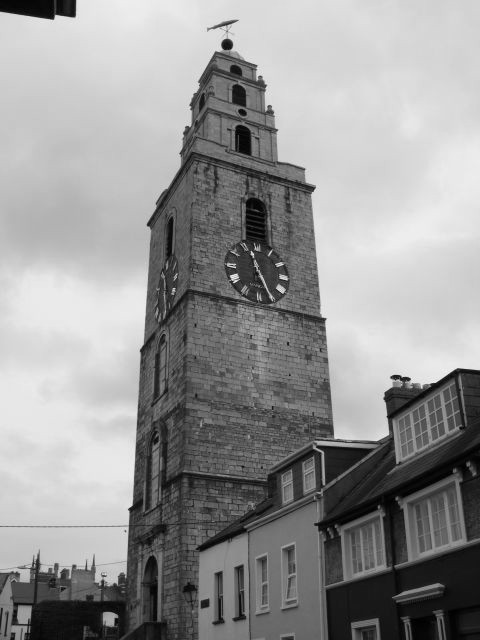
\includegraphics[height=.5\textheight]{img/Shandon_bells_cork.McCarron.grey.jpg}
  \caption[
    Classical Time. The \emph{Four Faced Liar}, Shandon Bells, Cork
  ]{
    A celebrated example of \emph{classical} time measurement (and measurement errors) in Cork~City
    (Shandon Bells, St. Anne's Church).
    These four clocks
    may famously
    indicate slightly different times from each other.
    % ``Each side of the tower also contains a clock face.
    % Installed in 1847 and affectionately known as the
    % `four-faced liar', the hands on the east and west run slightly fast, especially in windy weather.
    % This is probably because they are so very large
    % (only Big Ben in London has larger clock faces).''
    \parencite{McCarron, CorkStrolls}
  }
  %\vspace{3\baselineskip}
  \label{fig:ShandonBells}
\end{figure}
\end{savenotes}